\documentclass[a4paper, 12pt, conference]{IEEEtran}
\usepackage[utf8]{inputenc}
\usepackage[style=ieee]{biblatex}
\usepackage[numbered]{bookmark}
\usepackage{hyperref}
\usepackage{graphicx}
\usepackage{textcomp}
\usepackage{tikz}
\usepackage{amsmath}
\usepackage{amssymb}
\usepackage{mathtools}
\usepackage{booktabs}
\usepackage{subcaption}
\usepackage[ruled,vlined]{algorithm2e}
\usepackage{xcolor}

\title{CS-464 Term Project Final Report \\ Breakout Atari\texttrademark{} Game with Reinforcement Learning}
\author{\IEEEauthorblockA{Group 4}\IEEEauthorblockN{Abdullah Arda Aşçı (21702748), Alim Toprak Fırat (21600587), \\ Atahan Yorgancı (21702349), Tuna Alikaşifoğlu (21702125)}}
\date{\today}
\bibliography{bibliography}
\hypersetup{colorlinks=true, allcolors=[rgb]{0.5, 0, 0.5}}

\DeclareMathOperator*{\argmax}{arg\,max}
\DeclareMathOperator*{\argmin}{arg\,min}

\begin{document}
\maketitle
\thispagestyle{plain}
\pagestyle{plain}

\section{Introduction}
Breakout is an arcade game that was published and developed by Atari, where the player is in control of a paddle on the \(x\)-axis and tries to break down each brick by handling a ball. At each time the ball touches to a brick, that particular brick is destroyed and the player gains a point, the game is won if all the bricks are destroyed. A sample position from the game is provided in~\autoref{fig:breakout_image}.

\begin{figure}[h]
    \centering{}
    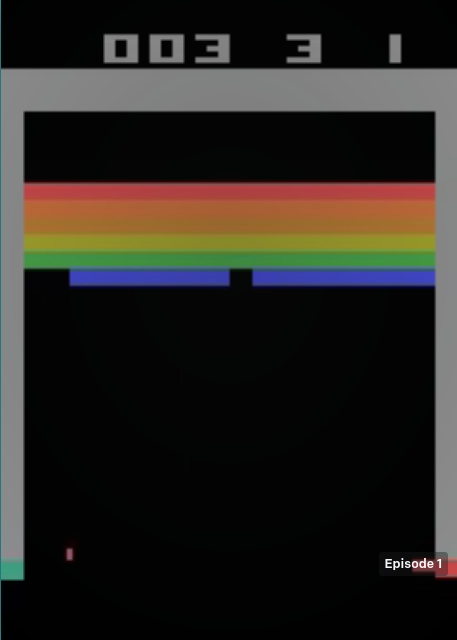
\includegraphics[width=\linewidth, height=0.33\textheight, keepaspectratio]{img/breakout.png}
    \caption{Sample Position from the Breakout Atari Game~\autocite{breakout_image}}~\label{fig:breakout_image}
\end{figure}

In order to obtain a model that can play the game and get better results than a random agent with the use of Supervised or Unsupervised Learning, a large amount of data needs to be generated. Reinforcement learning doesn't need any
data. In reinforcement learning, an agent who has a set of actions is trained in an environment using rewards or punishments considering the decisions of the agent in different situations.

In reinforcement learning, there is a \emph{environment}, which have different states changes at each time step, \(s_t \in S\), and a learning \emph{agent} who can observe the environment and then learns from the outcomes of it's actions, \(a_t \in A\). In reinforcement learning problems, the agents' decisions influence their own actions in proceeding steps, agents don't have any information of which actions to take in what situation and they try to maximize reward (or minimize punishment) by trying out different combinations in the set of actions.

One of the main challenges of RL is to build a model that can learn from the noisy and delayed environmental data. The latency between the incoming data forces training model to give a delayed input reaction and the delays add up to each other in a cascading manner. To overcome the delay problem significantly, rather than using computer vision to gather frames and analyze them one by one, a breakout game developed in such a way that all in-game data can be accessible to the model.

Another challenge is the incoming state data being highly correlated with the previously acquired ones, rather than being independent. To build a model which can perform well withing the high-dimensional correlated state space, a Deep Q-Network (DQN) is developed which combines reinforcement learning with deep neural networks. The many layered approach made it possible to build up more abstract representations of the correlated spatial data.

To be able to train our model, the action set, state space and rewards were defined for the Breakout game. The positive reward are defined as unit positive reward for every break of a brick. No negative rewards are defined. However, in order to stop the repetitive behavior, such as bouncing the ball of the wall and getting it back without breaking any bricks and exploiting the positive rewards, a random restart protocol is implemented, so that the model is pushed to explore rather than exploit.
\section{Problem Description}
The problem that we have is the utilization of deep reinforcement learning, with the specific model of convolutional neural networks, trained with Deep Q-Learning, whose input is raw pixel values, varying between \( \{0, 1, \dots, 255\} \), of a grayscale version of the image of the current state, and output is the most suitable action from the action space. The question that we would like to address is whether the trained agent can outperform a random agent, which takes random actions at each time step, and if so whether it can outperform a human agent that plays the game in the same settings.

\section{Methods}
As our project is to create a model with reinforcement learning, specifically DQN,
we do not have a predefined dataset. With this in mind, our methodology can be separated
into three parts.

\subsection{Reinforcement Learning}
Reinforcement Learning (RL) is a subset of Machine Learning (ML) where the
aim is to teach a model, called agent, via its interactions with the surrounding environment.
This method of learning requires no set of labeled or unlabeled data to be collected before
the learning actually starts. Instead the agent, typically a neural network,
is used for predicting the optimal action to be taken at each step based on its observation
and a reward is determined by the environment which is used for training the agent.
In RL, this environment is modeled as a Markov Decision Process (MDP)~\autocite{BUSONIU20188}.

\subsubsection{Markov Decision Process}
MDP is a mathematical framework based on Markov Chains for decision making processes
with inherent randomness. In Markov Decision Processes, we define:
\begin{itemize}
    \item \(S\): State Space (finite set),
    \item \(A\): Action Space (finite set),
    \item \(A_s\): Set of actions available at state \(s\),
    \item
          \(P^a_{ss'} = P_a(s,s') = P(s_{t+1} = s' \;|\; s_t = s, a_t = a)\) is the probability of action \(a\) in state \(s\) leading to state \(s'\),
    \item \(R_a(s, s')\): Reward received after transitioning from \(s\) to \(s'\).
\end{itemize}

\subsubsection{Markov Property}
For RL agents to work with MDPs we need the environment to be fully observable,
meaning that state \(s\) must capture all the characteristics of the environment.
In more technical terms, any state is \(S\) must satisfy the Markov Property which is defined as.
\begin{equation}
    P[s_{t+1} \;|\; s_t] = P[s_{t+1} \;|\; s_1, \ldots, s_t]
\end{equation}
This property essentially enables the environment to be memoryless which is required for
Markov Chains and more importantly its extension MDPs.

\subsubsection{Policy}
The objective in an MDP is to optimize the \textit{policy} of the decision making algorithm.
Here, we define the function \(\pi(s)\) that outputs the action chosen by the decision maker
based on the current state \(s\). This optimization mainly done by maximizing the cumulative
reward function. This function can be expressed as:
\begin{equation}
    G_t = \sum^{\infty}_{t=0}{\gamma^t R_a(s_t, s_{t+1})},\;
\end{equation}
where \(0\leq \gamma \leq 1\) is the discount factor. The equation above introduces the concept of \textit{discount factors}. This parameter is quite important as it is one of the hyperparameters of RL training loops. It is useful for avoiding cyclic behavior and infinite returns, and representing an exponentially increasing uncertainty for the future time steps.

Moreover, the policy that maximizes the function given above is regarded as as the
\textit{optimal policy} and denoted as \(\pi^*(s)\). It should be noted that this optimal policy is not necessarily unique.

\subsubsection{State-Value Function}
The state-value function, or just value function, is denoted by \(V_\pi(s)\). It is the expected return stating from state \(s\) and following policy \(\pi \) of an MDP\@. In most applications, it is used to evaluate how good being in a state is. It is mathematically expressed as:
\begin{equation}
    V_\pi(s) = E_\pi[G_t \;|\; s_t = s]
\end{equation}
As can be seen in the equation above, calculating the cumulative reward function is required
to find the value function of a state. This can be decomposed into a recursive function
as the current reward plus the discounted value function of the successor by utilizing
the Bellman Equation.
\begin{equation}
    V_\pi(s) = E_\pi[R_{t+1} + \gamma V_\pi(s_{t+1}) \;|\; s_t = s]
\end{equation}
With this done, we now define the state-value function that is produced by the optimal
policy \(\pi^*\) as the \textit{optimal state-value function}. In mathematical terms:
\begin{equation}
    V_*(s) = \max_\pi{V_\pi(s)}
\end{equation}

\subsubsection{Action Value Function}
The action value function, also called the Q-function, is the expected return starting from state \(s\), taking action \(a\), and then following policy \(\pi \). This is expressed as:
\begin{equation}
    Q_\pi(s,a) = E_\pi[G_t \;|\; s_t = s, a_t = a]
\end{equation}
Similar to the state-action function, we can also decompose this into a recursive function by redefining
\begin{equation}
    G_{t} = R_{t+1} + \gamma Q_\pi(s_{t+1}, a_{t+1}),
\end{equation}
and define the optimal action-value function as:
\begin{equation}
    Q_*(s,a) = \max_\pi{Q_\pi(s,a)}
\end{equation}

\subsubsection{Finding the Optimal Policy}
In all MDPs, three conditions are satisfied:
\begin{itemize}
    \item An optimal policy \(\pi^*\) exists (not necessarily unique),
    \item Optimal policy achieves the optimal state-value function
          \begin{equation}
              V_{\pi^*}(s) = V_*(s)
          \end{equation}
    \item Optimal policy achieves the optimal action-value function
          \begin{equation}
              Q_{\pi^*}(s,a) = Q_*(s, a)
          \end{equation}
\end{itemize}
These three assumptions can be used to shows that finding the optimal policy
\(\pi^*\) to solve the MDP can be done by maximizing over \(Q_*(s,a)\) with:
\begin{equation}
    \pi_*(a | s) =
    \begin{cases}
        1 & \text{if }\argmax_{a}{Q_*(s,a)} \\
        0 & \text{otherwise}
    \end{cases}
\end{equation}
This equation essentially means that finding the optimal policy can be done by
following the path given by \(Q_*(s,a)\) assuming that the optimal Q function is known~\autocite{mnih2013playing}.

\subsection{Neural Networks}
Artificial Neural Networks (ANNs), or simply Neural Networks (NNs), are
machine learning models that are loosely based on real life neurons and their connections.
Although the theoretical work for these types of models were mostly developed in mid
20\textsuperscript{th} century, the applications of them were quite limited considering
the computational power required for the necessary calculations.

\begin{figure}[h]
    \centering{}
    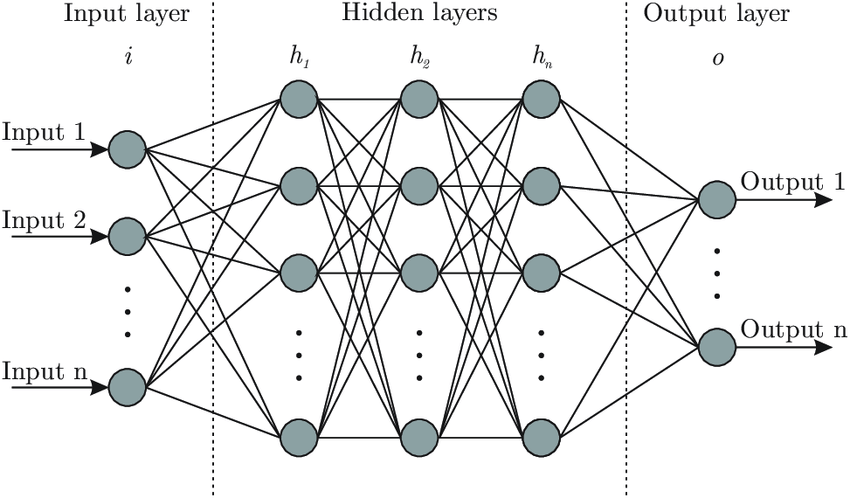
\includegraphics[width=\linewidth, height=0.3\textheight, keepaspectratio]{img/ann.png}
    \caption{A Basic ANN Structure~\autocite{buseyarentekin}}~\label{fig:ANN}
\end{figure}

In our project, the observation provided to the RL agent compromises of screenshots of
the game's graphics. Therefore, the NN we used is made up of mainly convolutional layers
for image processing with smaller fully connected layers at the end for decision making.
The entire neural network used is:
\begin{enumerate}
    \item Convolutional Layer: 32 filters,
    \item ReLu Activation Layer,
    \item Convolutional Layer: 64 filters,
    \item ReLu Activation Layer,
    \item Convolutional Layer: 64 filters,
    \item ReLu Activation Layer,
    \item Fully Connected Layer: 512 wide,
    \item ReLu Activation Layer,
    \item Fully Connected Layer: 4 wide
\end{enumerate}

\subsection{Deep Q Learning (DQN)}
The standard Q learning algorithm uses the training episodes to fill up a Q table where
each value corresponds to a specific action taken in a specific state. This method
functions properly when the amount of state action pairs are relatively low.
For example, the ``Cliff Walking Problem'', shown below, is simple enough that a Q table would be the feasible. In fact, the table would only have between 160 to 192 entries depending on  how the environment is defined.

\begin{figure}[h]
    \centering{}
    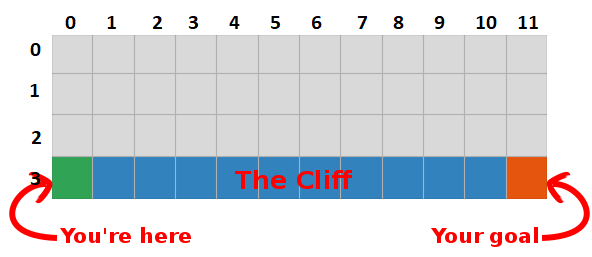
\includegraphics[width=\linewidth, height=0.3\textheight, keepaspectratio]{img/cliff_walking.png}
    \caption{Cliff Walking Problem~\autocite{Cliff_photo}}~\label{fig:CliffWalk}
\end{figure}


For more complicated environments, this approach quickly loses its feasibility.
In those cases, like what we have in Breakout, a neural network is used as a
nonlinear function approximator to replace the table. In DQN, the nn provides a
mapping from the give state \(s\), to the Q function of all possible actions in that
state \(Q(s,\underline{a})\).\\
The training loop of our network has a few additional, but still standard, features.
These are:
\begin{enumerate}
    \item
          \(\epsilon \)-greedy Policy: To simulate \textit{exploration}, the action will be chosen randomly with probability \(\epsilon \),
    \item Experience Replay Memory: To combat the unstable nature of deep reinforcement
          learning, a circular memory with a set size will be used to reduce the correlations
          between the sequence of observations used in every training batch.
    \item Target Network: An additional \textit{target network} is used to increase the
          stability of the learning.
\end{enumerate}
The final learning algorithm is given in~\autoref{algo:dqn} in~\autoref{app:dqn}.
\section{Results}
The agent was trained for 100000 episodes with random restarts every 20000 episodes. For evaluating the performance the agent average game length, mean \(Q\) value, mean reward, and mean loss is recorded. Results from one random restarts is shown in ~\autoref{fig:results} in~\autoref{app:results}. From the figures we can conclude that the agent improves its knowledge about the game nearly every episode. The graphs are not smoothed out, even tough the trajectory is clearly upwards for received reward, and as the agent explores the reward fluctuates.

\section{Discussion}
 {
  \color{red}
  Interpretation and discussion of the results.
 }

\section{Conclusion}
All in all, we successfully implemented a deep reinforcement learning architecture using convolutional neural networks, trained with Deep Q-Learning, whose input is raw pixel values, varying between \( \{0, 1, \dots, 255\} \), of a grayscale version of the image of the current state, and output is the most suitable action from the action space. As we demonstrated in our final presentation demo, our trained agent outperforms the random agent with less than an hour of training. As demonstrated, our own group members also played the game using the keyboard agent, although none of the group members can perform more than \(20\) in any of the trials. In this context, the trained agent outperforms every group member with the score of \(28\). Therefore, the answer to our initial question is yes! The trained agent with the specified model can outperform both random and human agents.

Throughout the project, we learned the basic approaches of reinforcement learning. We learned that by using CNNs and DQNs, it is possible to learn control policies directly from high-dimensional sensory input using reinforcement learning. The resultant agent is satisfactory to respond our question with ``yes''. In addition to basic theoretical approach, we also had the chance to interact with a practical issue that we were not expecting to face. While we were trying to adjust the exploration versus exploitation hyperparameter, \(\varepsilon \), we faced with an issue that we later learned it is called the credit assignment problem. The credit assignment problem means that it can happen that we choose an action, and we only win or lose hundreds of actions later, leaving us with no idea of as to which of our actions led to this win or lose, thus, making it difficult to learn from our actions~\autocite{mnih2013playing}. We learned that solely increasing the training duration does increase the performance of the agent. We learned that in order to overcome this credit assignment pitfall, using random restarts actually increases the performance of the agent, by adjusting the exploration versus exploitation problem in the direction of exploration.

As the future work of the project, performance of the agent can be increased by changing the deep neural network architecture and increasing the training duration. During our project, we have encountered with more complex approaches like double DQNs, Never Give-Up (NGU), etc. Experimentation on these approaches can be expressed as potential future work. Furthermore, these approaches can be generalized as \textit{DeepMind}'s \texttt{Agent57} to provide trained agents for \(57\) atari games~\autocite{agent57}.


\clearpage
\printbibliography{}

\newpage
\begin{appendices}
    \section{Contribution}
    \begin{table}[h]
        \centering
        \caption{Task Sharing}\label{tab:task_sharing}
        \begin{tabular}{rl}\toprule
            \textbf{Student}   & \textbf{Task}                              \\\midrule
            Abdullah Arda Aşçı & Setting OpenAI, and developing             \\
                               & wrappers for \texttt{gym} environment.     \\
                               & Training \& testing with different         \\
                               & hyperparameters.                           \\
            \midrule
            Atahan Yorgancı    & Background research about RL               \\
                               & and DQN\@. Implementation of artificial    \\
                               & agent. Cloud based training training       \\
                               & \& testing with different hyperparameters. \\
            \midrule
            Alim Toprak Fırat  & Background research about RL               \\
                               & and Q-Learning. Training \& testing        \\
                               & with different hyperparameters.            \\
            \midrule
            Tuna Alikaşifoğlu  & Developing CLI for running, and            \\
                               & training using \texttt{gym} environment.   \\
                               & Implementation of DQN\@. Training \&       \\
                               & testing with different                     \\ \bottomrule
        \end{tabular}
    \end{table}
\end{appendices}

\end{document}
